\newpage
\section{Expected Shortfall}
\subsection{Tail Value at Risk (TVaR)}
\textbf{Overview} : One common shortcoming of Value at Risk is the inability to capture the behavior of the distribution beyond $V_X^p$ (as illustrated in figure \ref{fig:var-shortcoming}). Hence, one way to remedy this shortcoming is to taking the average of Value at Risk beyond the level $p$.
\begin{figure}[ht]
    \centering
    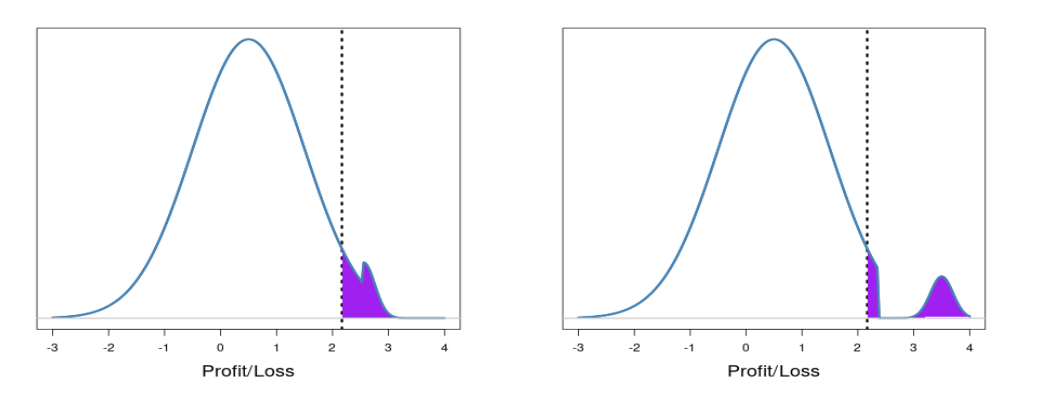
\includegraphics[width=\textwidth]{figures/var_shortcoming.png}
    \caption{Two distributions having the same $V_X^{0.95} = 2.145$ (figure sampled from \cite{book:privault})}
    \label{fig:var-shortcoming}
\end{figure}

\begin{definition}[Tail Value at Risk (TVaR)]
    The Tail Value at Risk (TVaR) of a random variable $X$ at the level $p\in(0,1)$ is defined by the following average:
    \begin{align*}
        \boxed{
            TV_X^p = \frac{1}{1-p} \int_p^1 V_X^qdq
        }
    \end{align*}

    \noindent Note that $p \to V_X^p$ is a non-decreasing function (Proposition \ref{prop:properties_of_var}). Therefore, we always have:
    \begin{align*}
        TV_X^p = \frac{1}{1-p}\int_p^1 V_X^{\bf q}dq \ge \frac{1}{1-p}\int_p^1 V_X^{\bf p}dq = V_X^p
    \end{align*}
\end{definition}

\subsection{Conditional Tail Expectation (CTE)}
\textbf{Overview} : Conditional Tail Expectation is another measure that takes into account "what happens beyond $V_X^p$. However, instead of taking the uniform average as Tail Value at Risk, Conditional Tail Expectation takes the conditional expectation of $X$ conditioned on the event that $X > V_X^p$.

\begin{definition}[Conditional Expectation]
    Given a random variable $X$ and an event $A$ such that $P(A)>0$. The conditional expectation of $X$ given the event $A$ is defined as:
    \begin{align*}
        \mathbb{E}[X|A] = \frac{1}{P(A)}\mathbb{E}[X\1{A}]
    \end{align*}
\end{definition}

\begin{definition}[Conditional Tail Expectation (CTE)]
    Given a random variable $X$ such that $P(X>V_X^p)>0$ at a level $p\in (0,1)$. The \textbf{Conditional Tail Expectation} of $X$ at level $p$ is defined as:
    \begin{align*}
        \boxed{
            CTE_X^p = \mathbb{E}\Big[
                X \Big| X > V_X^p
            \Big] = \frac{\mathbb{E}[X\1{X>V_X^p}]}{P(X>V_X^p)}
        }
    \end{align*}

    \noindent The Conditional Tail Expectation can be written as a Distortion Risk Measure $CTE_X^p=\mathbb{E}\Big[ Xf_X(X)\Big]$ with the distortion function:
    \begin{align*}
        \boxed{
            f_X(x) = \frac{1}{P(X>V_X^p)}\1{x>V_X^p}
        }
    \end{align*}
\end{definition}

\begin{proposition}{$CTE_X^p - V_X^p$}{cte_and_var_diff}
    For any $p\in(0,1]$, we have $CTE_X^p > \mathbb{E}[X]$ and $CTE_X^p > V_X^p$. Specifically:
    \begin{align*}
        CTE_X^p = \mathbb{E}\Big[ X\Big|X>V_X^p \Big] = V_X^p + \mathbb{E}\Big[(X-V_X^p)^+ | X > V_X^p\Big]
    \end{align*}
\end{proposition}

\begin{proof*}[Proposition \ref{prop:cte_and_var_diff}]
    We have :
    \begin{align*}
        \mathbb{E}\Big[ X | X > V_X^p \Big] 
            &= \frac{1}{P(X>V_X^p)}\mathbb{E}\Big[ X\1{X > V_X^p} \Big] \\
            &= \frac{1}{P(X>V_X^p)}\Bigg[ \mathbb{E}\Big[ (X - V_X^p) \1{X > V_X^p} \Big] + V_X^p\mathbb{E}\Big[ \1{X > V_X^p} \Big] \Bigg] \\
            &= \frac{1}{P(X>V_X^p)}\Bigg[ \mathbb{E}\Big[ (X - V_X^p) \1{X > V_X^p} \Big] + V_X^pP(X>V_X^p) \\
            &= V_X^p + \frac{1}{P(X>V_X^p)} \mathbb{E}\Big[ (X - V_X^p) \1{X > V_X^p} \Big] \\
            &= V_X^p + \mathbb{E}\Big[ X - V_X^p | X > V_X^p \Big]
    \end{align*}
\end{proof*}

\begin{proposition}{When $CTE_X^p=TV_X^p$}{when_cte_equal_tvar}
    When $P(X=V_X^p)=0$, meaning there is no discontinuity at $V_X^p$, then we have:
    \begin{align*}
        P(X=V_X^p)=0 \iff CTE_X^p = TV_X^p
    \end{align*}
\end{proposition}

\begin{proof*}[Proposition \ref{prop:when_cte_equal_tvar}]
    By figure \ref{fig:lemma3.1_illustration}, we can see that when $P(X=V_X^p)=0$, we have, with probability one, $P(V_X^U > V_X^p) = P(V_X^U \ge V_X^p) = P(U \ge p)$. Hence:
    \begin{align*}
        CTE_X^p &= \mathbb{E}\Big[ X | X > V_X^p\Big] \\
        &= \frac{1}{P(X>V_X^p)}\mathbb{E}\Big[ X\1{X > V_X^p} \Big] \\
        &= \frac{1}{P(U \ge p)}\mathbb{E}\Big[ X\1{U \ge p} \Big] \\
        &= \frac{1}{P(U \ge p)}\mathbb{E}\Big[ V_X^U\1{U \ge p} \Big] \\
        &= \frac{1}{1-p} \int_p^1 V_X^qdp = TV_X^p
    \end{align*}
\end{proof*}

\begin{definition}[Gaussian CTE (G-CTE)]
    Given $X\sim \mathcal{N}(\mu_X, \sigma_X^2)$, we have:
    \begin{align*}
        \boxed{
        CTE_X^p = \mu_X + \frac{\sigma_X}{1-p}\varphi(V_Z^p) = \mu_X + \frac{\sigma_X}{(1-p)\sqrt{2\pi}}\exp\Bigg( -\frac{(V_Z^p)^2}{2} \Bigg)
        }
    \end{align*}
    \noindent Or we can write:
    \begin{align*}
        CTE_X^p = \mu_X + \frac{\sigma_X}{(1-p)\sqrt{2\pi}}\exp\Bigg( -\frac{(q_Z^p)^2}{2} \Bigg)
    \end{align*}

    \noindent $\varphi(.)$ is the standard normal probability density function.
\end{definition}

\subsection{Expected Shortfall (ES)}
\begin{definition}[Expected Shortfall (ES)]
    Given a random variable $X$, the \textbf{Expected Shortfall (ES)} at the level $p \in (0,1)$ is defined by
    \begin{align*}
        \boxed{
            ES_X^p = V_X^p + \frac{1}{1-p} \mathbb{E}\Big[ 
                (X - V_X^p)\1{X\ge V_X^p}
            \Big]
        }
    \end{align*}

    \noindent The Expected Shortfall (ES) can be written as a Distortion Risk Measure $ES_X^p=\mathbb{E}\Big[ Xf_X(X) \Big]$ defined as:
    \begin{align*}
        \boxed{
            f_X(x) = \frac{1}{1-p}\Bigg( 
                \1{X > V_X^p} + \1{P(X=V_X^p) > 0}\1{X=V_X^p}\frac{1-p-P(X>V_X^p)}{P(X=V_X^p)}
            \Bigg)
        }   
    \end{align*}
    \noindent\newline This can be deduced from proposition \ref{prop:alternative_dfn_es} below.
\end{definition}

\begin{proposition}{Altenative definition of $ES_X^p$}{alternative_dfn_es}
    The Expected Shortfall (ES) at level $p\in(0,1)$ can be written as:
    \begin{align*}
        ES_X^p = \frac{1}{1-p}\mathbb{E}[X\1{X\ge V_X^p}] + \frac{V_X^p}{1-p}\Big(1-p-P(X\ge V_X^p)\Big)
    \end{align*}
\end{proposition}

\begin{proof*}[Proposition \ref{prop:alternative_dfn_es}]
    We have:
    \begin{align*}
        ES_X^p 
            &= V_X^p + \frac{1}{1-p}\mathbb{E}\Big[ (X - V_X^p)\1{X\ge V_X^p} \Big] \\
            &= V_X^p + \frac{1}{1-p}\mathbb{E}\Big[X-V_X^p \Big| X\ge V_X^p \Big] P(X\ge V_X^p) \\
            &= V_X^p + \frac{P(X\ge V_X^p)}{1-p}\Bigg\{ \mathbb{E}\Big[ X| X \ge V_X^p \Big] - V_X^p \Bigg\} \\
            &= V_X^p + \frac{P(X\ge V_X^p)}{1-p}\Bigg\{ \frac{1}{P(X\ge V_X^p)} \mathbb{E}\Big[ X\1{X\ge V_X^p} \Big] - V_X^p \Bigg\} \\
            &= \frac{1}{1-p}\mathbb{E}\Big[ X\1{X\ge V_X^p} \Big] + V_X^p \Big( 1 - \frac{P(X\ge V_X^p)}{1-p} \Big) \\
            &= \frac{1}{1-p}\mathbb{E}\Big[ X\1{X\ge V_X^p} \Big] + \frac{V_X^p}{1-p}\Big( 1 - p - P(X\ge V_X^p) \Big)
    \end{align*}
\end{proof*}

\begin{corollary}{$ES_X^p$ when $P(X=V_X^p) = 0$}{es_when_continuous}
    As a direct consequence of Proposition \ref{prop:alternative_dfn_es}, we have:
    \begin{align*}
        P(X=V_X^p) = 0 \iff ES_X^p = CTE_X^p
    \end{align*}

    \noindent By proposition \ref{prop:when_cte_equal_tvar}, we can even have:
    \begin{align*}
        P(X=V_X^p) = 0 \iff ES_X^p = CTE_X^p = TV_X^p
    \end{align*}
\end{corollary}

\begin{proof*}[Corollary \ref{coro:es_when_continuous}]
    When $P(X=V_X^p) = 0$, we have $p=F_X(V_X^p)=P(X\le V_X^p)=P(X<V_X^p)$. Hence, by the definition of expected shortfall, we have:
    \begin{align*}
        ES_X^p 
        &= V_X^p + \frac{1}{1-p}\mathbb{E}\Big[ (X - V_X^p)\1{X\ge V_X^p} \Big] \\
        &= V_X^p + \frac{1}{1 - P(X \le V_X^p)}\mathbb{E}\Big[ (X - V_X^p)\1{X\ge V_X^p} \Big] \\
        &= V_X^p + \frac{1}{P(X > V_X^p)}\mathbb{E}\Big[ (X - V_X^p)\1{X\ge V_X^p} \Big] \\
        &= V_X^p + \frac{1}{P(X > V_X^p)}\mathbb{E}\Big[ X - V_X^p \Big| X \ge V_X^p \Big] P(X\ge V_X^p) \\
        &= V_X^p + \frac{1}{P(X > V_X^p)}\mathbb{E}\Big[ X - V_X^p \Big| X > V_X^p \Big] P(X > V_X^p) \\
        &= V_X^p + \mathbb{E}\Big[ X - V_X^p \Big| X > V_X^p \Big] \\
        &= \mathbb{E}\Big[ X \Big| X > V_X^p \Big] = CTE_X^p
    \end{align*}
\end{proof*}

\begin{proposition}{$ES_X^p$ and $TV_X^p$ for any $p\in(0,1)$}{es_tv_any_p}
    This proposition proves a much stronger result than Corollary \ref{coro:es_when_continuous}. For any $p\in(0,1)$ (not just when $P(X = V_X^p) = 0$), we have:
    \begin{align*}
        ES_X^p = TV_X^p = \frac{1}{1-p}\int_p^1 V_X^qdq
    \end{align*}
\end{proposition}

\begin{proof*}[Proposition \ref{prop:es_tv_any_p}]
    We first prove the following claim:

    \begin{subproof}{\newline Claim 1 : $V_X^p\Big(1-p-P(X\ge V_X^p) \Big)=-\mathbb{E}\Big[ X\1{ ( X\ge V_X^p ) \cap (U<p)} \Big]$}
        For $U\sim Uniform(0,1)$, note that:
        \begin{align*}
            P(U \ge p) &= 1 - p = \mathbb{E}\Big[ \1{U \ge p} \Big] \\
            P(X \ge V_X^p) &= \mathbb{E}\Big[ \1{X \ge V_X^p} \Big]
        \end{align*}

        \noindent (Note that it is tempting to conclude that $P(X\ge V_X^p)=P(V_X^U \ge V_X^p) = P(U\ge p)$. However, this is not true by lemma \ref{lem:x_equal_vx_power_u} because we can have $V_X^{p_1}\ge V_X^{p_2}$ for $p_1<p_2$ if there is discontinuity between $p_1$ and $p_2$). 

        \noindent \newline Now, we have:
        \begin{align*}
            V_X^p\Big( 1 - p - P(X\ge V_X^p) \Big) 
                &= V_X^p\Bigg( 
                    \mathbb{E}\Big[ \1{U\ge p} \Big] - \mathbb{E}\Big[ \1{X \ge V_X^p} \Big]
                \Bigg) \\
                &= - V_X^p \mathbb{E}\Big[ \1{X \ge V_X^p} - \1{U\ge p} \Big] \\ 
                &= - V_X^p \mathbb{E}\Big[ \1{(X \ge V_X^p)\setminus (U \ge p)} \Big] \\ 
                &= - V_X^p \mathbb{E}\Big[ \1{(X \ge V_X^p)\cap (U < p)} \Big] \\ 
        \end{align*}

        \noindent \newline As illustrated in figure \ref{fig:lemma3.1_illustration}, when the event $(V_X^U \ge V_X^p)\cap (U<p)$ occurs, we have $X=V_X^p$. Hence, we can also write:
        \begin{align*}
            V_X^p\Big( 1 - p - P(X\ge V_X^p) \Big) 
                &= - V_X^p \mathbb{E}\Big[ \1{(X \ge V_X^p)\cap (U < p)} \Big] \\ 
                &= - \mathbb{E}\Big[ X \1{(X \ge V_X^p)\cap (U < p)} \Big]
        \end{align*}
    \end{subproof}

    \begin{subproof}{\newline Claim 2 : $ES_X^p = TV_X^p$}
        From the above, we have:
        \begin{align*}
            ES_X^p &= \frac{1}{1-p}\mathbb{E}\Big[ X\1{X\ge V_X^p}\Big] + \frac{V_X^p}{1-p}\Big( 1 - p - P(X\ge V_X^p) \Big) \ \ \ \text{(By proposition \ref{prop:alternative_dfn_es})} \\
            &= \frac{1}{1-p}\Bigg( \mathbb{E}\Big[ X\1{X\ge V_X^p}\Big] - \mathbb{E}\Big[ X \1{(X \ge V_X^p)\cap (U < p)} \Big] \Bigg) \\
            &= \frac{1}{1-p}\mathbb{E}\Big[ X\1{(X\ge V_X^p) \cap (X\ge V_X^p)^c \cup (U \ge p)}\Big] \\
            &= \frac{1}{1-p}\mathbb{E}\Big[ X\1{U \ge p}\Big] \\
            &= \frac{1}{1-p}\mathbb{E}\Big[ V_X^U\1{U \ge p}\Big] \\
            &= \frac{1}{1-p}\int_p^1 V_X^qdq = TV_X^p
        \end{align*}
    \end{subproof}
\end{proof*}

\begin{theorem}{Coherence of $ES_X^p$ and $TV_X^p$}{coherence_es_tv}
    \textbf{Expected shortfall (ES)} and \textbf{Tail Value at Risk (TVaR)} are coherent risk measures. The \textbf{Conditional Tail Expectation (CTE)} is generally not coherent (incoherent when $P(X=V_X^p)>0$). 
\end{theorem}

\begin{proof*}[Theorem \ref{thm:coherence_es_tv}]
    Since Expected Shortfall (ES) and Tail Value at Risk (TVaR) are the same for any $p\in(0,1)$, we can use either measure to prove coherence. In this proof, we will use Tail Value at Risk (TVaR).

    \begin{subproof}{\newline (i) Monotonicity}
        Let $X, Y$ be random variables such that $X \le Y$. We have:
        \begin{align*}
            TV_X^p = \frac{1}{1-p}\int_p^1 V_X^qdq \le \frac{1}{1-p}\int_p^1 V_Y^qdq = TV_Y^p \ \ \text{(Since VaR is monotone)}
        \end{align*}
    \end{subproof}
    
    \begin{subproof}{\newline (ii) Positive homogeneity and translation invariance}
        Let $\lambda > 0$ and $\mu \ge 0$, we have:
        \begin{align*}
            TV_{\mu + \lambda X}^p &= \frac{1}{1-p}\int_p^1 V_{\mu + \lambda X}^q dq \\
            &= \int_p^1 \Big( \mu + \lambda V_X^q \Big)dq \\
            &= \mu + \frac{\lambda}{1-p}\int_p^1 V_X^qdq \\
            &= \mu + \lambda TV_X^p
        \end{align*}
    \end{subproof}

    \begin{subproof}{\newline (iii) Sub-additivity}
        Since the Expected Shortfall (ES) can be written as a Distortion Risk Measure with the following distortion function:
        \begin{align*}
            f_X(x) = \frac{1}{1-p}\Bigg( 
                \1{X > V_X^p} + \1{P(X=V_X^p) > 0}\1{X=V_X^p}\frac{1-p-P(X>V_X^p)}{P(X=V_X^p)}
            \Bigg)
        \end{align*}

        \noindent\newline We have:
        \begin{align*}
            (1 - p)(ES_{X+Y}^p - ES_X^p - ES_Y^p) 
                &= (1 - p)\Bigg( \mathbb{E}\Big[ (X+Y)f_{X+Y}(X + Y)\Big] - \mathbb{E}\Big[ Xf_X(X) \Big] - \mathbb{E}\Big[ Yf_Y(Y) \Big] \Bigg) \\
                &= (1 - p)\Bigg( \mathbb{E}\Big[ X\Big(f_{X+Y}(X+Y) - f_X(X)\Big) \Big] + \mathbb{E}\Big[ Y\Big(f_{X+Y}(X+Y) - f_Y(Y)\Big)\Big] \Bigg) \\
                &\le V_X^p \mathbb{E}\Big[ f_{X+Y}(X+Y) - f_X(X)\Big] + V_Y^p \mathbb{E}\Big[ f_{X+Y}(X+Y) - f_Y(Y) \Big] \\
                &= V_X^p(1 - 1) + V_Y^p(1-1) = 0 \\
                \implies ES_{X+Y}^p &\le ES_X^p + ES_Y^p
        \end{align*}
    \end{subproof}
\end{proof*}

\subsection{Conclusion (Asset risk measures)}
\textbf{Remark} : As a concluding remark, we have the following
\begin{align*}
    \text{When } P(X = V_X^p) 
    \begin{cases}
        = 0   &\implies TV_X^p = ES_X^p    = CTE_X^p \\ \\
        \ne 0 &\implies TV_X^p = ES_X^p \ne CTE_X^p
    \end{cases}
\end{align*}

\noindent\newline \textbf{Summary of asset risk measures} :
\begin{table}[ht]
\begin{center}
\resizebox{\textwidth}{!}{
\begin{tabular}{l | r | r | r }
\toprule
\textbf{Risk measure} & \textbf{Definition} & \textbf{Gaussian} & \textbf{Others} \\
    \midrule\midrule
    \textbf{VaR ($V_X^p$)}          
        & $\inf\Big\{ x \in \mathbb{R} : P(X\le x) \ge p \Big\}$                    
        & $\mu_X + \sigma_Xq_Z^p$    
        & N/A
        \\
    \midrule

    \textbf{TVaR ($TV_X^p$)}         
        & $\frac{1}{1-p}\int_p^1 V_X^qdq$                    
        & N/A     
        & N/A
        \\
    \midrule
    
    \textbf{ES ($ES_X^p$)}           
        & $V_X^p + \frac{1}{1-p}\mathbb{E}\Big[ (X-V_X^p)\1{X\ge V_X^p} \Big]$                    
        & N/A        
        & $\frac{1}{1-p}\Big( \mathbb{E}[X\1{X\ge V_X^p}] + V_X^p(1-p-P(X\ge V_X^p)) \Big)$
        \\
    \midrule
    
    \textbf{CTE ($CTE_X^p$)}          
        & $\mathbb{E}\Big[ X \Big| X > V_X^p \Big]$                   
        & $\mu_X + \frac{\sigma_X}{1-p}\varphi(q_Z^p)$ 
        & $V_X^p + \mathbb{E}\Big[ X - V_X^p | X > V_X^p \Big]$
        \\
    \bottomrule\bottomrule
\end{tabular}}
\end{center}
\end{table}

\noindent \textbf{Coherence of asset risk measures} : 
\begin{table}[ht]
\resizebox{\textwidth}{!}{\begin{tabular}{@{}lllll@{}}
\toprule
\textbf{Risk measure} & \textbf{Monotonicity} & \textbf{Homogeneity} & \textbf{Sub-additivity} & \textbf{Coherence} \\
\midrule\midrule
\textbf{VaR}          & \color{green} Yes     & \color{green} Yes    & \color{red} No          & \color{red} No     \\
\textbf{TVaR}         & \color{green} Yes     & \color{green} Yes    & \color{red} No          & \color{red} No     \\
\textbf{ES}           & \color{green} Yes     & \color{green} Yes    & \color{green} Yes       & \color{green} Yes  \\
\textbf{CTE}          & \color{green} Yes     & \color{green} Yes    & \color{green} Yes       & \color{green} Yes  \\ 
\bottomrule\bottomrule
\end{tabular}}
\end{table}